%%
%
% ARQUIVO: main.tex
%
% VERSÃO: 1.1
% DATA: Abril de 2016
% AUTOR: Coordenação PPgSC
% 
%  Arquivo tex principal relatório de Avaliação de Trabalho de Dissertação.
%  Este arquivo SÓ PRECISA SER MODIFICADO NA PARTE DE CONTEÚDO:
%
%    a. arquivos secao-02.tex; secao-03.tex; refs.bib.
%
%%

% -----
% CLASSE DO DOCUMENTO DO RELATÓRIO DE TRABALHO DE DISSERTAÇÃO
% -----
\documentclass{seminario}

% -----
% PACOTES LATEX USADOS NO RELATÓRIO DE TRABALHO DE DISSERTAÇÃO
% -----
\usepackage[brazilian]{babel}
\usepackage[utf8]{inputenc}
\usepackage[T1]{fontenc}

\usepackage{amsmath}
\usepackage{graphicx}
\usepackage{tabularx}
\usepackage{float}
\usepackage{color}
\usepackage{amsfonts,amssymb}
\usepackage[authoryear]{natbib}

\usepackage{enumitem}
\usepackage{rotating}
\usepackage{lipsum}
\usepackage{lastpage}
\usepackage{stringstrings}
\usepackage{pgffor}

% -----
% MARGENS DO DOCUMENTO DO RELATÓRIO DE TRABALHO DE DISSERTAÇÃO
% -----
\usepackage{geometry}
\geometry{
	a4paper,
	left=25mm,
	right=25mm,
	top=25mm,
	bottom=30mm,
	headheight=0mm,
	headsep=0mm,
}

% -----
% DECLARAÇÕES AUXILIARES PARA REFERÊNCIAS
%
%  Diferencia \citet e \citep de acordo com a NBR 10520:2002
% -----
\DeclareRobustCommand{\NATand}{;}
\DeclareRobustCommand{\NATetal}{et~al.}
\makeatletter
\renewcommand{\NAT@nmfmt}[1]{%
  \ifNAT@swa\expandafter\MakeUppercase
  \else\DeclareRobustCommand{\NATand}{ e}\expandafter\@firstofone\fi{{\NAT@up #1}}%
}
\makeatother

% -----
% AMBIENTE DE FIGURAS DO RELATÓRIO DE TRABALHO DE DISSERTAÇÃO
%
%  A classe do documento está configurada SOMENTE para figuras no formato EPS.
%  Logo, use PREFERENCIALMENTE este tipo de arquivo.
%
%    a. os arquivos das figuras devem estar no diretório 'img'
% -----
\graphicspath{{./img/}}

% -----
% INÍCIO DO DOCUMENTO DO RELATÓRIO DE TRABALHO DE DISSERTAÇÃO
% -----
\begin{document}

% -----
% DADOS DO RELATÓRIO DE TRABALHO DE DISSERTAÇÃO
%  ALTERAR o arquivo dados-seminario.tex
% -----
%%
%
% ARQUIVO: dados-seminario.tex
%
% VERSÃO: 1.1
% DATA: Abril de 2016
% AUTOR: Coordenação PPgSC
% 
%  Arquivo tex com os dados acerca do relatório de Avaliação de Trabalho de Dissertação.
%
%
%%

%%% AUTOR DA APRESENTAÇÃO DE SEMINÁRIO (Nome completo)
\autor{Nycolas Wenderson da Silva dos Santos}

%%% CÓDIGO DO AUTOR DA APRESENTAÇÃO DE SEMINÁRIO
\codigoautor{SC 23202}

%%% POSTO DO AUTOR DA APRESENTAÇÃO DE SEMINÁRIO
% ---
%  se o autor é CIVIL, REMOVA ESTA LINHA
%  se o autor é MILITAR, coloque CORRETAMENTE o POSTO aqui
% ---
%\postoautor{1 Ten}

%%% TITULO DO TRABALHO DE DISSERTAÇÃO
\titulo{ATRIBUIÇÃO DE ALGORITMOS DE CRIPTOGRAFIA LEVE EM CENÁRIO
CIPHERTEXT-ONLY VIA APRENDIZADO DE MÁQUIN}

%%% TÍTULO ANTERIOR DO TRABALHO DE DISSERTAÇÃO
% ---
%  se o título do trabalho NÃO foi alterado desde a última
%     apresentação (Proposta ou Seminário), REMOVA ESTA LINHA
%  se o título do trabalho FOI ALTERADO, coloque aqui o ANTIGO
%     título COMPLETO do trabalho:
% ---
%\titantigo{Título Anterior Completo do Trabalho de Dissertação}

%%% DATA DA APRESENTAÇÃO DE SEMINÁRIO (formato {dd}{Mmmmm}{aaaa})
\dataapresentacao{07}{Julho}{2026}

%%% ÁREA DE CONCENTRAÇÃO DO TRABALHO DE DISSERTAÇÃO
% ---
%  VER SITE do PPGSC para ver as Áreas de Concentração do Programa.
%  Em 2016 só existe uma Área de Concentração:
%     Ciência da Computação
% ---
\area{Ciência da Computação}

%%% LINHA DE PESQUISA DO TRABALHO DE DISSERTAÇÃO
% ---
%  VER SITE do PPGSC para ver as Linhas de Pesquisa do Programa.
%  Em 2016 só existem três Linhas de Pesquisa:
%     Metodologia da Computação
%     Sistemas de Computação
%     Engenharia de Sistemas e Informação
% ---
\linha{Sistemas de Computação}

%%% ORIENTADOR DO TRABALHO DE DISSERTAÇÃO
% ---
%  CAMPO 1: Nome completo
%  CAMPO 2: D (para D.Sc.); P (para Ph.D.); ou qualquer coisa (inclusive VAZIO) - o que for escrito aparecerá no documento
% ---
\orientador{Jose Antonio Moreira Xéxeo}{D}

%%% POSTO DO ORIENTADOR DO TRABALHO DE DISSERTAÇÃO
% ---
%  se o orientador é CIVIL, REMOVA ESTA LINHA
%  se o orientador é MILITAR, coloque CORRETAMENTE o POSTO aqui:
%     pode ser: 1 Ten; Cap; Maj; Ten Cel; Cel
% ---
\postoorientador{Ten Cel}

%%% CO-ORIENTADOR DO TRABALHO DE DISSERTAÇÃO
% ---
%  se NÃO HOUVER co-orientador, REMOVA ESTA LINHA
%  preenchimento idêntico a \orientador{}{}
% ---
%\coorientador{Nome Completo do Co-orientador}{P}

%%% POSTO DO CO-ORIENTADOR DO TRABALHO DE DISSERTAÇÃO
% ---
%  se NÃO HOUVER co-orientador, REMOVA ESTA LINHA
%  caso contrário
%    se o co-orientador é CIVIL, REMOVA ESTA LINHA
%    se o co-orientador é MILITAR, coloque CORRETAMENTE o POSTO aqui:
%       pode ser: 1 Ten; Cap; Maj; Ten Cel; Cel
% ---
%\postocoorientador{Cap}

%%% COORDENADOR DE PÓS-GRADUAÇÃO
% ---
%  CAMPO 1: Nome completo
%  CAMPO 2: D (para D.Sc.); P (para Ph.D.); ou qualquer coisa (inclusive VAZIO) - o que for escrito aparecerá no documento
% ---
\coord{Gabriela Moutinho de Souza Dias}{P}

%%% POSTO DO COORDENADOR DE PÓS-GRADUAÇÃO
% ---
%  se o Coordenador de PG é CIVIL, REMOVA ESTA LINHA
%  se o Coordenador de PG é MILITAR, coloque CORRETAMENTE o POSTO aqui:
%     pode ser: 1 Ten; Cap; Maj; Ten Cel; Cel
% ---
\postocoord{Maj}

%%% CHEFE DA SEÇÃO (SE/8)
\chefe{Julio Cesar Duarte}

%%% POSTO DO CHEFE DA SEÇÃO (SE/8)
% ---
%  se o Chefe é CIVIL, REMOVA ESTA LINHA
%  se o Chefe é MILITAR, coloque CORRETAMENTE o POSTO aqui:
%     pode ser: 1 Ten; Cap; Maj; Ten Cel; Cel
% ---
\postochefe{Cel}



% -----
% PARTE PRÉ-TEXTUAL DO RELATÓRIO DE TRABALHO DE DISSERTAÇÃO
% -----
\makecapa
\maketitle

\parindent 0.75cm


% -----
% PARTE DE CONTEÚDO DE SEU RELATÓRIO DE TRABALHO DE DISSERTAÇÃO
%
% Alterar o conteúdo dos arquivos secao-02.tex / secao-03.tex
% -----
% -----
% ARQUIVO: secao-02.tex
% VERSÃO: 1.1
% DATA: Abril de 2016
%
% SEÇÃO DE INTRODUÇÃO DO RELATÓRIO DO TRABALHO DE ACOMPANHAMENTO
%
% NÃO MEXA NAS SEÇÕES, SOMENTE EDITE O CONTEÚDO.
% -----

\chapter{Introdu\c{c}\~{a}o}

Este relatório descreve a trajetória completa das atividades de pesquisa desenvolvidas até o momento na dissertação de mestrado. A pesquisa investiga se criptogramas produzidos por quatro algoritmos de criptografia leve, padronizados ou finalistas do processo do NIST, Ascon-AEAD128, GIFT-COFB, Grain-128AEAD e Schwaemm256-128, podem ser atribuídos ao algoritmo que os gerou por meio de aprendizado de máquina, quando o observador dispõe apenas do texto cifrado, sem acesso à chave, ao nonce ou ao texto em claro. O conjunto de algoritmos candidatos é conhecido de antemão, de modo que a tarefa consiste em decidir qual entre os quatro produziu um determinado criptograma.

Essa tarefa se situa entre outras que a literatura também trata como distinção, e que diferem entre si pela distribuição de referência adotada em cada caso. O distinguisher de indistinguibilidade compara a saída de uma cifra com uma sequência uniformemente aleatória, e corresponde à própria definição de segurança do esquema. O distinguisher diferencial compara pares de criptogramas gerados a partir de textos em claro com diferença conhecida contra pares aleatórios, e pressupõe que o adversário conheça ou controle a relação entre as entradas; \citet{gohr_2019} introduziu a versão neural dessa abordagem sobre Speck32/64, e \citet{shen_2024_giftascon} a aplicaram a GIFT-128 e Ascon, com acurácia de 99,36\% sobre 7 das 40 rodadas do GIFT-128 e de 69,25\% sobre 4 das 12 rodadas da permutação do Ascon, em ambos os casos sobre a primitiva isolada e com rodadas reduzidas. Os testes estatísticos de aleatoriedade, como a suíte NIST SP 800-22, comparam uma sequência isolada com a hipótese de uniformidade; oito dos vinte e um estudos mapeados na revisão sistemática desta pesquisa os empregam como extratores de características para identificação de algoritmo, uso que pressupõe que cada cifra se afaste da aleatoriedade de maneira própria e reprodutível.

A tarefa desta dissertação adota uma referência distinta das três anteriores: a comparação é feita entre as saídas de dois algoritmos, cada uma individualmente indistinguível de uma sequência aleatória, sobre as primitivas completas e no modo de criptografia autenticada em que operam na prática. Como a indistinguibilidade computacional é transitiva, criptogramas individualmente indistinguíveis de uma sequência uniforme também o são entre si, de modo que a hipótese nula corresponde à previsão teórica para o cenário avaliado. Um resultado positivo, nesse enquadramento, apontaria para a presença de assinaturas estruturais ou de implementação situadas fora do modelo idealizado, como diferenças de comprimento de tag e de nonce, padding ou particularidades do código de referência, possibilidades que o protocolo experimental precisa controlar.

As atividades realizadas incluem: (i) implementação e validação de wrappers criptográficos de referência para os quatro algoritmos



As atividades realizadas incluem: (i) implementação e validação de wrappers criptográficos de referência para os quatro algoritmos: Ascon, GIFT-COFB, Grain-128AEAD e Schwaemm256-128; (ii) construção de um pipeline de geração de datasets de 180.000 amostras encadeadas entre os quatro algoritmos e dois controles; (iii) extração de 641 características estatísticas dos criptogramas, organizadas em doze famílias, e implementação de um pipeline de seleção em múltiplos estágios; (iv) condução de experimentos de classificação sobre os algoritmos criptograficos leves, com múltiplos modelos e representações, abrangendo características estatísticas clássicas (Random Forest, SVM, LinearSVC e XGBoost), representações latentes extraídas por redes neurais convolucionais unidimensionais e bidimensionais, e uma estratégia híbrida que combina ambas as fontes de informação; (v) implementação de controles positivos e negativos para validar a capacidade do pipeline de detectar sinais estruturais quando presentes;  

O resultado central obtido até o momento, no recorte submetido ao SBSeg 2026, é a confirmação da hipótese nula (H0) em todas as quatro frentes experimentais conduzidas: sob protocolo experimental rigoroso, nenhum dos modelos avaliados, independentemente da representação utilizada, foi capaz de distinguir criptogramas com desempenho estatisticamente superior ao acaso. 
 

Nota: Foi utilizada Inteligência Artificial Generativa (ChatGPT ) como ferramenta de apoio na redação e atualização deste relatório.

















\section{Objetivo}
a dissertação tem como objetivo identificar, entre Ascon-AEAD128, GIFT-
COFB, Grain-128AEAD e Schwaemm256-128, o algoritmo de criptografia leve (LWC)
gerador de um criptograma observado, considerando exclusivamente o modelo de acesso
somente a criptogramas.
Como objetivos específicos, pretende-se:

\begin{enumerate}
\item  desenvolver a cadeia de processamento de atribuição algorítmica (pré-processamento,
extração/seleção de características e treinamento de modelos) para classificar a
origem do criptograma;
\item construir um dataset reprodutível de benchmark para aprendizado de máquina.

\end{enumerate}

\section{Problemas de Pesquisa}
Diferenças de projeto e de implementação entre algoritmos de criptografia leve podem deixar assinaturas estatísticas residuais no criptograma, exploráveis por aprendizado de máquina. Se essas assinaturas permitirem identificar o algoritmo gerador a partir do tráfego cifrado observado passivamente, um atacante reduz seu espaço de busca, direciona a exploração de vulnerabilidades específicas e pode realizar fingerprinting de dispositivos em ecossistemas IoT heterogêneos, mesmo sem acesso à chave. A literatura de identificação de algoritmos criptográficos por ML reporta acurácias elevadas para cifras convencionais, mas poucos estudos avaliam esquemas AEAD leves padronizados por entidades internacionalmente reconhecidas, e principalmente algoritmos selecionados pelo NIST.

\section{Contribuições Esperadas}
Esta dissertação contribui em três frentes. A primeira é metodológica: um protocolo de geração e avaliação que neutraliza os mecanismos de vazamento identificados na revisão de literatura, reaproveitamento de chave entre treino e teste e seleção de características fora do laço de validação cruzada, aplicado a quatro algoritmos e dois controles cifrados de forma encadeada com a mesma chave, o mesmo nonce e o mesmo texto em claro. A segunda é a evidência empírica: cinco representações independentes do criptograma, descritores estatísticos, duas representações aprendidas por CNN, fusão híbrida e um Transformer hierárquico, entre elas réplicas fiéis de técnicas documentadas na literatura para outros cenários de classificação de cifras, agora testadas em um cenário mais realista e sem vazamento entre treino e teste, avaliadas sob os mesmos controles positivo e negativo, o que configura uma verificação de segurança ampla, sensível a diferentes tipos de assinatura residual que uma única representação poderia deixar passar, e permite comparar a sensibilidade de cada uma em vez de depender de um único classificador para sustentar a conclusão. A terceira é o artefato: um dataset reprodutível de 180.000 criptogramas, com manifesto de geração e validação de integridade documentada, disponível como benchmark para trabalhos futuros de identificação algorítmica, independentemente do resultado encontrado aqui.
% -----
% ARQUIVO: secao-03.tex
% VERSÃO: 1.1
% DATA: Abril de 2016
%
% SEÇÃO DE ACOMPANHAMENTO DO TRABALHO DE DISSERTAÇÃO
%
% NÃO MEXA NAS SEÇÕES, SOMENTE EDITE O CONTEÚDO.
% -----

\chapter{Acompanhamento do Trabalho}
Esta seção detalha as tarefas já realizadas, as tarefas em andamento e a cumprir, os resultados parciais e a avaliação do andamento do trabalho.


\begin{tarefac} Revisão de literatura 
A tarefa inicial foi a condução de duas revisões de literaturas, a primeira, com o foco na precisão teve o objetivo de mapear o problema especifico que seria alvo da atual dissertação. Seu objetivo foi mapear artigos sobre identificação algorítmica de cifras a partir de criptogramas, organizada em quatro eixos: estudos que estabelecem, com classificadores clássicos, que descritores de bytes cifrados carregam informação suficiente para distinguir algoritmos; a transição para arquiteturas de aprendizado profundo nessa mesma tarefa; um eixo transversal sobre mecanismos de vazamento em protocolos de avaliação; e a lacuna que a dissertação ocupa. Seis trabalhos foram revisados em profundidade: \citet{mello_xexeo_2018}, sete algoritmos de bloco clássicos em ECB/CBC; \citet{yuan2022}, o ensemble HKNNRF sobre estatísticas NIST SP 800-22; \citet{sikdar_kule_2024}, um transformador BERT sobre cifras majoritariamente clássicas; e, na linha de distinguishers neurais para criptanálise diferencial, \citet{gohr_2019}, \citet{benamira_2021} e \citet{su2025neural}. Nenhum dos seis trabalhos avalia o par Ascon-AEAD128/GIFT-COFB nem esquemas AEAD padronizados, o que estabeleceu a lacuna inicial de cobertura desta pesquisa.

A segunda RSL teve como objetivo fortalecer a dissertação, ao buscar novas técnicas e possibilidades de melhoria, ampliando a fundamentação teórica e fornecendo maior respaldo científico às escolhas metodológicas adotadas na pesquisa. Foi conduzida, segundo o protocolo de \citet{kitchenham_charters_2007} e relatada conforme o PRISMA 2020, sobre identificação de algoritmos criptográficos por aprendizado de máquina a partir de ciphertexts. A busca cobriu cinco bases (Scopus, IEEE Xplore, ACM Digital Library, SpringerLink e Web of Science) e foi encerrada em agosto de 2026. Após deduplicação, 864 registros únicos foram triados por título e resumo no Rayyan, dos quais 51 avançaram para leitura de texto completo e 21 estudos, publicados entre 2016 e 2026, foram incluídos na análise, os 30 restantes foram considerados adjacentes, sendo separados para estudo futuro. A extração cobriu objetivo, algoritmos avaliados, modelos, representação, protocolo experimental e limitações de cada estudo, sem meta-análise, já que os trabalhos usam datasets, algoritmos e definições de classe distintos entre si. O achado central é a ausência de cobertura: nenhum dos 21 estudos avalia Ascon, GIFT-COFB ou as demais finalistas do processo de padronização de criptografia leve do NIST, e nenhum avalia modo de criptografia autenticada. Um segundo achado, transversal a oito dos estudos incluídos, é a degradação de desempenho por granularidade da tarefa, com indício, levantado por \citet{tan_ji_2016}, de que o comprimento de bloco compartilhado entre algoritmos, não sua identidade, é o que efetivamente se separa nesses experimentos.


\end{tarefac}






\begin{tarefac}Implementação da infraestrutura criptográfica de referência
Foram implementados wrappers em Python, Interface) no modo API out-of-line, para as implementações de referência em C do Ascon-AE via CFFI (C Foreign FunctionAD128 e do GIFT-COFB. Essa abordagem permite invocar diretamente as funções de cifragem e decifragem sem o overhead de gerenciamento de processos externos, ao mesmo tempo em que preserva integralmente o código de referência oficial, sem qualquer modificação. A corretude de ambas as implementações foi validada por meio dos vetores de teste oficiais (Known Answer Tests, KATs) distribuídos pelo NIST. 

Posteriormente infraestrutura de wrappers foi estendida para mais dois algoritmos de criptografia leve, que foram selecionados entre os 10 finalistas NIST, por terem uma arquitetura diferente dos já implementados, trazendo assim uma maior diversidade, ambos foram implementados seguindo a mesma abordagem via CFFI sobre as implementações de referência em C. Grain-128AEAD, uma cifra de fluxo baseada em LFSR e NFSR, difere dos dois algoritmos anteriores por ter nonce e tag menores, 96 e 64 bits respectivamente. Schwaemm256-128, uma construção em esponja da família SPARKLE baseada em operações ARX, tem o maior nonce do conjunto, 256 bits. Os 1.089 vetores de teste dos quatro algoritmos foram validados com sucesso em sua totalidade, com tempo de execução inferior a 10 milissegundos.  
\end{tarefac}
 
\begin{tarefac}
 Foi construído um dataset encadeado de 180.000 criptogramas, a partir de 300 chaves e 100 amostras de texto em claro por chave, cifradas pelos quatro algoritmos de criptografia leve avaliados e por dois controles, AES-ECB e um gerador de números pseudoaleatórios, com a mesma chave, o mesmo nonce e o mesmo texto em claro entre os seis. O texto em claro é fixo em 64 KB por amostra, com 80\% extraído do Standardized Project Gutenberg Corpus e 20\% de imagens em tons de cinza do ImageNet-1k, sorteados por amostra. As chaves foram geradas por um mecanismo determinístico validado contra vetores de teste oficiais (CAVP). O dataset foi submetido a cinco verificações de integridade: unicidade de nonces por chave, uniformidade de bytes por teste qui-quadrado (taxa de rejeição abaixo de 10\% ao nível de significância de 5\%), taxa de compressão média próxima de 1,0, verificação de decifragem ponta a ponta sobre 100 amostras aleatórias e manifesto com hash SHA-256 dos binários, seeds e parâmetros de geração. O veredito da validação foi de aprovação em todos os critérios.


\end{tarefac}
 
 
 
\begin{tarefac}Extração e seleção de características estatísticas

O extrator de características foi ampliado de seis para doze famílias e de 307 para 641 dimensões medidas, mantendo as seis famílias originais, histograma de bytes, entropia, n-gramas, autocorrelação, complexidade e espectro de Fourier, e acrescentando seis novas: suíte completa de testes de aleatoriedade do NIST SP 800-22, momentos estatísticos, distribuição de peso de Hamming, densidade espectral por Welch, blocos de bits e características da região da tag de autenticação. A extração foi reimplementada para processar o dataset em fluxo, em vez de carregar o parquet inteiro em memória, viabilizando sua aplicação às 180.000 amostras do v2. Sobre esse vetor ampliado, foi implementado um pipeline de seleção em cinco estágios, aplicado exclusivamente à partição de treinamento de cada fold da validação cruzada. O primeiro normaliza cada característica por z-score, corrigindo o viés que famílias de escalas absolutas muito diferentes, como contagens de histograma e valores de entropia, introduziam no estágio seguinte. O segundo aplica um limiar de variância, descartando características quase constantes entre as amostras. O terceiro ordena as características por informação mútua com o rótulo. O quarto aplica mRMR (minimum Redundancy Maximum Relevance), que define o conjunto final ao equilibrar relevância individual para o rótulo e redundância mínima entre as características escolhidas entre si. O quinto é o Boruta, que compara a importância de cada característica real contra cópias embaralhadas dela mesma.
\end{tarefac}
 
 
 
\begin{tarefac}
Modelagem e avaliação experimental - características estatísticas clássicas:
Foram avaliados quatro classificadores sobre as 307 características estatísticas (Caminho A): Random Forest, SVM com kernel RBF (otimizado por busca em grade sobre 16 combinações de hiperparâmetros), LinearSVC e XGBoost. A avaliação seguiu protocolo estatístico rigoroso, incluindo F1-macro como métrica principal, intervalos de confiança via bootstrap (1.000 reamostragens) e teste de McNemar para comparações pareadas entre modelos, com correção de Bonferroni. Os quatro classificadores convergiram para F1-macro próximo de 0,50, compatível com a hipótese nula de indistinguibilidade.
\end{tarefac}
 
 
 
\begin{tarefac} Implementação dos caminhos experimentais e da consolidação estatística
Foram implementados os seis caminhos experimentais do protocolo v2 e o script de consolidação estatística entre eles. O Caminho A reúne os classificadores clássicos (Random Forest, SVM RBF, LinearSVC, XGBoost, Regressão Logística) sobre as 641 características extraídas, acrescidos de réplicas fiéis de três técnicas publicadas na literatura, o ensemble HKNNRF de \citet{yuan2022}, o XGB-LGBM sobre peso de Hamming de \citet{zhao_hamming_2023} e o Transformer E20 de \citet{yuan_e20_2026}. Os Caminhos B e C extraem representações latentes por CNN unidimensional e bidimensional, respectivamente; o Caminho D combina as três representações, estatística e as duas latentes, em um classificador híbrido; o Caminho E é um Transformer hierárquico com atenção local e global sobre os bytes crus; e o Caminho F é um meta-classificador por stacking sobre as saídas dos cinco caminhos anteriores. 
\end{tarefac}





 
\section{Tarefas a Cumprir}
 \begin{tarefanc}Execução dos Caminhos B, C e E
 
 Está planejada a execução dos Caminhos B, C e E, que extraem e classificam a partir de representações latentes de CNN unidimensional, CNN bidimensional e do Transformer hierárquico próprio, respectivamente, sobre as 180.000 amostras de criptogramas.
\end{tarefanc}

\begin{tarefanc}Execução dos Caminhos D e F
Os Caminhos D e F, o classificador híbrido sobre a concatenação das representações estatística e latentes, e o meta-classificador por stacking sobre as saídas dos cinco caminhos anteriores, dependem da conclusão dos Caminhos B, C e E e serão executados na sequência.
\end{tarefanc}
 
\begin{tarefanc}Consolidação estatística e redação final

Após a execução dos seis caminhos, será realizada a consolidação estatística entre eles, com correção de Benjamini-Hochberg para taxa de descoberta falsa entre as múltiplas comparações, teste de McNemar pareado com correção de Bonferroni e estratificação de erro por classe. Os capítulos da dissertação relativos a resultados, discussão e conclusão serão redigidos a partir dessa consolidação, hoje pendente da execução completa dos caminhos experimentais.
\end{tarefanc}
 


\section{Resultados Parciais}
Nos experimentos de classificação conduzidos, nenhum modelo atingiu desempenho estatisticamente superior ao acaso (F1-macro $\approx$ 0,50) na tarefa de distinguir Ascon-AEAD128 de GIFT-COFB, com intervalos de confiança bootstrap consistentemente cobrindo o valor de referência do acaso. Esse resultado confirma a hipótese nula (H0) e é consistente com as garantias teóricas de segurança esperadas para esquemas AEAD modernos.



\section{Cronograma Atualizado}

O cronograma para o desenvolvimento das atividades relacionadas a este trabalho de dissertação de mestrado pode ser visto na Figura 3.1.

% #CRONOGRAMA
\begin{figure}[!h]
	\centering
	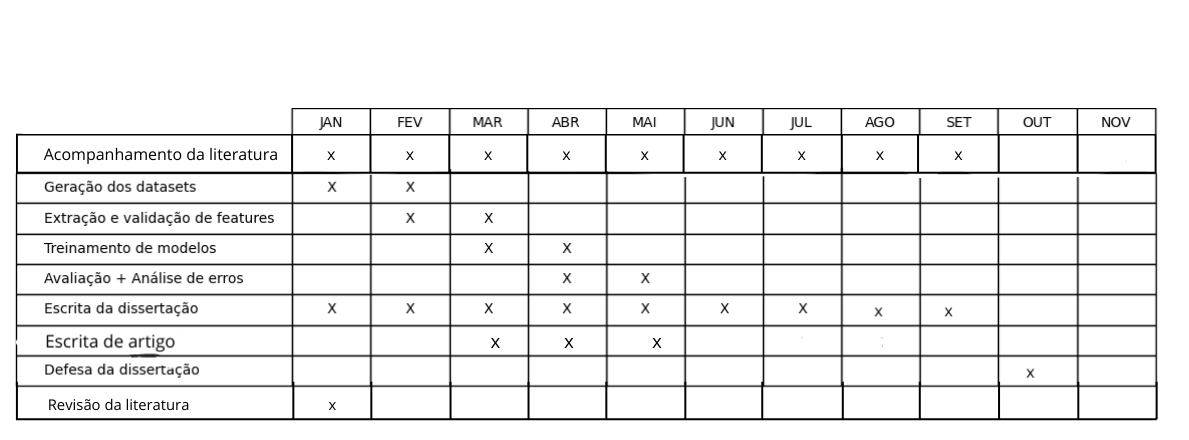
\includegraphics[width=0.9\textwidth]{img/x.png}
	\caption{Cronograma de Disserta\c{c}\~{a}o.}
	\label{fig:cronograma}
\end{figure}

\section{Avaliação do Andamento do Trabalho}



% -----
% PARTE DE REFERÊCIAS BIBLIOGRÁFICAS DO TRABALHO DE DISSERTAÇÃO
%
%  As referências do Trabalho de Dissertação devem estar no arquivo refs.bib
%  Devem seguir o formato bibtex - ver Manual-Referencias.pdf para mais detalhes.
% -----
\bibliographystyle{seminario}
\bibliography{refs}


% -----
% PARTE DE ASSINATURAS DE SEU TRABALHO DE DISSERTAÇÃO
% -----
\preparatitulos
\makeassinaturas


% -----
% FIM DO DOCUMENTO DE SEU TRABALHO DE DISSERTAÇÃO
% -----
\label{theend}
\end{document}
